  


%%%%%%%%%%%%%%%%%%%%%%%%%%%%%%%%%%%%%%%%%%%%%%%%%%%%%%%%%%%%%%%%%%%%%%%%%%%%%
%%%%%%%%%%%%%%%%%%%%%%%%%%%%%%%%%%%%%%%%%%%%%%%%%%%%%%%%%%%%%%%%%%%%%%%%%%%%%
%%%%%%%%%%%%%%%%%%%%%%%%%%%%%%%%%%%%%%%%%%%%%%%%%%%%%%%%%%%%%%%%%%%%%%%%%%%%%
 

                                                                             
\begin{figure*}[t]
\begin{center}
\resizebox{.8\textwidth}{!}{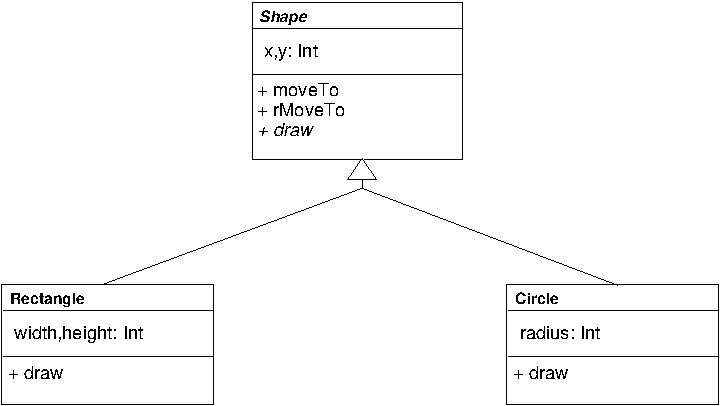
\includegraphics{shapes.pdf}}
\end{center}
\vspace{-33\in}
\caption{The `shapes' benchmark for subtype polymorphism}
\label{F:shapes}
\end{figure*}
                                                                             

 
%%%%%%%%%%%%%%%%%%%%%%%%%%%%%%%%%%%%%%%%%%%%%%%%%%%%%%%%%%%%%%%%%%%%%%%%%%%%%
%%%%%%%%%%%%%%%%%%%%%%%%%%%%%%%%%%%%%%%%%%%%%%%%%%%%%%%%%%%%%%%%%%%%%%%%%%%%%
%%%%%%%%%%%%%%%%%%%%%%%%%%%%%%%%%%%%%%%%%%%%%%%%%%%%%%%%%%%%%%%%%%%%%%%%%%%%%
 

 
\section{The Shapes benchmark}
\label{S:shapes}


Let us now explore the so-called `shapes benchmark'.\footnote{See the
multi-lingual collection `OO Example Code' by Jim Weirich at
\url{http://onestepback.org/articles/poly/}; see also an even heavier
collection `OO Shape Examples' by Chris Rathman at
\url{http://www.angelfire.com/tx4/cus/shapes/}.}  This benchmark (or
OO coding scenario) has a history in evaluating encodings of
subtype polymorphism. The classes that are involved in the
scenario are shown in Fig.~\ref{F:shapes}. There is an abstract class
(or an interface) @Shape@, and their are two subclasses @Rectangle@
and @Circle@. The coding scenario is the following: place different
shape object of different subclasses in a collection and iterate over
the collection to draw each shape object; the drawing
functionality varies per subclass.

We will show that the OOHaskell encoding pleasantly mimics the C++
encoding, while any remaining deviations are appreciated. We will also
discuss some variation points, once we have identified our prime
encoding. Finally, there are various possible encodings of the
scenario that do not deliver an image of Haskell as a true OO language
(including the one in Rathman's suite;
\url{http://www.angelfire.com/tx4/cus/shapes/haskell.html}). We do not
have space to discuss such non-OOHaskell encodings, but we refer to
this paper's source code distribution~\cite{OOHaskell} instead.



%%%%%%%%%%%%%%%%%%%%%%%%%%%%%%%%%%%%%%%%%%%%%%%%%%%%%%%%%%%%%%%%%%%%%%%%%%%%%
%%%%%%%%%%%%%%%%%%%%%%%%%%%%%%%%%%%%%%%%%%%%%%%%%%%%%%%%%%%%%%%%%%%%%%%%%%%%%
%%%%%%%%%%%%%%%%%%%%%%%%%%%%%%%%%%%%%%%%%%%%%%%%%%%%%%%%%%%%%%%%%%%%%%%%%%%%%



\subsection{The C++ reference solution}

We omit the code for the classes of shapes, rectangles and
circles. This is all trivial from a C++ perspective: we use a
pure virtual method for @draw@ in the class @Shape@, which is then
implemented differently in the classes @Rectangle@ and @Circle@.

Here is C++ code to set up an array of (two) shapes:

\begin{code}
   Shape *scribble[2];
   scribble[0] = new Rectangle(10, 20, 5, 6);
   scribble[1] = new Circle(15, 25, 8);
\end{code}

\noindent
We use an array rather than a collection type. We could employ a
collection type from C++'s Standard Template Library with similar
convenience. Here is a for-loop over the array in our C++ code:

\begin{code}
   for (int i = 0; i < 2; i++) {
      scribble[i]->draw();
      scribble[i]->rMoveTo(100, 100);
      scribble[i]->draw();
   }
\end{code}

\noindent
That is, we draw each element, move it relatively to its
origin, and draw it again. If the @draw@ method prints
`progress messages' about what is being drawn, we may see the
following output:

\begin{code}
 Drawing a Rectangle at:(10,20), width 5, height 6
 Drawing a Rectangle at:(110,120), width 5, height 6
 Drawing a Circle at:(15,25), radius 8
 Drawing a Circle at:(115,125), radius 8
\end{code}

\noindent
(Any OO language with parametric polymorphism, or at least polymorphic
arrays, should allow similarly concise code. In a typed language
without parametric polymorphism, we would need to bother about unsafe
down-casts when processing the aggregated objects. Likewise, untyped
languages would risk `message-not-understood' errors.)



%%%%%%%%%%%%%%%%%%%%%%%%%%%%%%%%%%%%%%%%%%%%%%%%%%%%%%%%%%%%%%%%%%%%%%%%%%%%%
%%%%%%%%%%%%%%%%%%%%%%%%%%%%%%%%%%%%%%%%%%%%%%%%%%%%%%%%%%%%%%%%%%%%%%%%%%%%%
%%%%%%%%%%%%%%%%%%%%%%%%%%%%%%%%%%%%%%%%%%%%%%%%%%%%%%%%%%%%%%%%%%%%%%%%%%%%%



\subsection{The OOHaskell transcription}

We also omit the Haskell values for the involved classes since we have
exercised pure virtual methods in Sec.~\ref{S:self}. We only
transcribe the collection code. We start a monadic @do@ sequence to
construct two shape objects~---~just as above:

\begin{code}
 myShapesOOP =
    do
       s1 <- mfix (rectangle (10::Int) (20::Int) 5 6)
       s2 <- mfix (circle (15::Int) 25 8)
       -- to be continued
\end{code}

\noindent
What's different? We use @mfix@ in place of @new@. We use curried
functions instead of C++'s comma notation.  We note that some
constructor arguments are annotated by the @Int@ type because we
preferred to eliminate the implicit polymorphism at this stage.

We continue the monadic @do@ sequence by building an `array' of
shapes:

\begin{code}
       let scribble :: [Shape Int]
           scribble = [narrow s1, narrow s2]
\end{code}

\noindent
In fact, we use a plain Haskell list. The type annotation for the
@scribble@ binding corresponds to the typed variable declaration in
the C++ code. However, the Haskell list construction differs from the
the C++ array construction as follows. In Haskell, we use an
explicit coercion operation, @narrow@ to prepare each shape object for
insertion into the homogeneous list. By contrast, such casting is
\emph{implicit} in the C++ code.

Regarding the class type @Shape@, we note that we have not used
\emph{any} explicit class types in the preceding sections. Mostly, we
do not need them because Haskell's type inference works
fine. (Programmers of C++ and of other mainstream languages have
the habit of writing down types for almost everything.) For the
purpose of \emph{casting}, we require such explicit types in
OOHaskell. They are necessary for steering explicit casting in the
view of programs that otherwise lack pervasive type annotations: So
here is the record type for @Shape@ objects:

\begin{code}
 type Shape a = Record (  (Proxy GetX    , IO a)
                      :*: (Proxy GetY    , IO a)
                      :*: (Proxy SetX    , a -> IO ())
                      :*: (Proxy SetY    , a -> IO ())
                      :*: (Proxy MoveTo  , a -> a -> IO ())
                      :*: (Proxy RMoveTo , a -> a -> IO ())
                      :*: (Proxy Draw    , IO ())
                      :*: HNil )
\end{code}

We finish up the monadic @do@ sequence by iterating over scribble:

\begin{code}
       mapM_ (\shape -> do
                           shape # draw
                           (shape # rMoveTo) 100 100
                           shape # draw)
             scribble
\end{code}

\noindent
Here we use the monadic @mapM_@ operation which only cares about the
effects of the monadic steps, throwing away results. This is really
the Haskell way of iterating over a list with effectful
functions~---~as the counterpart of the for-loop in the C++ code.



%%%%%%%%%%%%%%%%%%%%%%%%%%%%%%%%%%%%%%%%%%%%%%%%%%%%%%%%%%%%%%%%%%%%%%%%%%%%%
%%%%%%%%%%%%%%%%%%%%%%%%%%%%%%%%%%%%%%%%%%%%%%%%%%%%%%%%%%%%%%%%%%%%%%%%%%%%%
%%%%%%%%%%%%%%%%%%%%%%%%%%%%%%%%%%%%%%%%%%%%%%%%%%%%%%%%%%%%%%%%%%%%%%%%%%%%%



\subsection{Narrowing vs.\ heterogeneity vs.\ existentials}

We have employed narrowing to coerce all objects to a common
interface, in fact, to the \emph{same} record type. One might wonder
whether these coercions can be avoided altogether, or whether the
explicit conversions can also be made implicit even in OOHaskell. We
will discuss two techniques, but the conclusion will be that narrowing
is to be preferred.

The first technique is to collect the shape objects, as is, in a
\emph{heterogeneous} list rather than a homogeneous array or list. We
cannot construct such a list with the normal, polymorphic list datatype
constructor, but the \HList\ library comes again to our rescue. 
The scribble construction can now be performed without any
narrowing:

\begin{code}
       let scribble = s1 `HCons` (s2 `HCons` HNil)
\end{code}

\noindent
We cannot use ordinary list-processing function anymore, but the
\HList\ library mimics the normal list-processing API for @HList@s. So
there is also a heterogeneous variation on @mapM_@, namely @hMapM_@,
to be invoked as follows:

\begin{Verbatim}[fontsize=\small,commandchars=\\\{\}]
       hMapM_ (\undefined::FunOnShape) scribble
\end{Verbatim}

\noindent
The first argument of @hMapM_@ is not a function but rather a
\emph{type code}. This is necessary for technical reasons related to
the combination of rank-n polymorphism and ad-hoc
polymorphism.\footnote{A heterogeneous map function can encounter
entities of different types. Hence, its argument function must be
polymorphic on its own (which is different from the normal map
function). The argument function typically uses type classes (say,
ad-hoc polymorphism) to process the entities of different types. The
trouble is that the map function cannot possibly anticipate all the
constraints required by its argument function.  The type-code
technique moves the constraints from the type of the heterogeneous map
function to the interpretation site of the type codes.} The meaning of
each type code must be defined by a dedicated instance of an @Apply@
class for function application. Here is the declaration of the type
code @FunOnShape@ complete with its meaning:

\begin{code}
 data FunOnShape -- a type code only!
\end{code}

\begin{code}
instance ( HasField (Proxy Draw) r (IO ())
         , HasField (Proxy RMoveTo) r (Int -> Int -> IO ())
         )
      => Apply FunOnShape r (IO ())
  where
    apply _ x = do
                   x # draw
                   (x # rMoveTo) 100 100
                   x # draw
\end{code}

\noindent
The @Apply@ instance manifests encoding efforts that we didn't face
for the narrowing-based encoding. Now we have to list the
\emph{method-access constraints} (for ``\#'', i.e., @HasField@) in the
@Apply@ instance. Haskell's type-class system requires us to provide
proper bounds for the instance. One might argue that the form of these
constraints strongly resembles the method types listed in the class
type @Shape@. So one might wonder whether we can somehow use the full
class type in order to constrain the instance.  Haskell won't let us
do that in any reasonable way. (Constraints are not first-class
citizens in Haskell; we can't compute them from types or type
proxies~---~unless we were willing to rely on heavy encoding or
advanced syntactic sugar.) So we are doomed to manually infer such
method-access constraints for each such piece of polymorphic code.

The second technique for avoiding narrowing relies on placing shape
objects in \emph{existentially quantified envelopes}: we do not
coerce, but we wrap:

\begin{code}
       let scribble = [ WrapShape s1 , WrapShape s2 ]
\end{code}

\noindent
The declaration of the @WrapShape@ type depends on the function that
we want to apply to the opaque data. In our case, we can use the
normal @mapM_@ function again; we only need to unwrap the @WrapShape@
constructor prior to method invocations:

\begin{code}
       mapM_ ( \(WrapShape shape) -> do
                  shape # draw
                  (shape # rMoveTo) 100 100
                  shape # draw )
             scribble
\end{code}

\noindent
These operations have to be anticipated in the type bound for
@WrapShape@:

\begin{Verbatim}[fontsize=\small,commandchars=\\\{\}]
 data WrapShape =
  \Forall x. ( HasField (Proxy Draw) x (IO ())
       , HasField (Proxy RMoveTo) x (Int -> Int -> IO ())
       ) => WrapShape x
\end{Verbatim}

\noindent
It becomes evident that this result agrees with the heterogeneity
technique in terms of encoding efforts. In both cases, we need to
identify type-class constraints that correspond to the (potentially)
polymorphic method invocations.

Consequently, the narrowing technique is to be preferred.  We
\emph{could} hide narrowing by eschewing free-wheeling functional
programming and type inference. The required style and API would then
account for hidden narrowing. We do not favour such an approach for
various reasons. Abandoning type inference is in conflict with Haskell
native style.  Making casts implicit introduces the risk that the
programmer can accidentally pass an object of the wrong type.  Making
cast implicit hides the costs that come with casts; we prefer to see
the need for coercions clearly. (In fact, in the presence of multiple
inheritance of classes or interfaces, the implicit cast is absolutely
nontrivial, either for the compiler, or for the run-time system, or
both.)



%%%%%%%%%%%%%%%%%%%%%%%%%%%%%%%%%%%%%%%%%%%%%%%%%%%%%%%%%%%%%%%%%%%%%%%%%%%%%
%%%%%%%%%%%%%%%%%%%%%%%%%%%%%%%%%%%%%%%%%%%%%%%%%%%%%%%%%%%%%%%%%%%%%%%%%%%%%
%%%%%%%%%%%%%%%%%%%%%%%%%%%%%%%%%%%%%%%%%%%%%%%%%%%%%%%%%%%%%%%%%%%%%%%%%%%%%
